\documentclass[a4paper,11pt]{article}

\usepackage{cmap}					
\usepackage{mathtext} 				
\usepackage[T2A]{fontenc}			
\usepackage[utf8]{inputenc}			
\usepackage[english,russian]{babel}	

\usepackage{amsmath,amsfonts,amssymb,amsthm,mathtools}

\usepackage{euscript}	 
\usepackage{mathrsfs}


\usepackage{graphicx}  
\graphicspath{{images/}{images2/}} 
\setlength\fboxsep{3pt} 
\setlength\fboxrule{1pt} 
\usepackage{wrapfig} 

%Свои команды
\DeclareMathOperator{\Lin}{\mathrm{Lin}}
\DeclareMathOperator{\Linp}{\Lin^{\perp}}
\DeclareMathOperator*\plim{plim}
\DeclareMathOperator{\grad}{grad}
\DeclareMathOperator{\card}{card}
\DeclareMathOperator{\sgn}{sign}
\DeclareMathOperator{\sign}{sign}

\DeclareMathOperator*{\argmin}{arg\,min}
\DeclareMathOperator*{\argmax}{arg\,max}
\DeclareMathOperator*{\amn}{arg\,min}
\DeclareMathOperator*{\amx}{arg\,max}
\DeclareMathOperator{\cov}{Cov}
\DeclareMathOperator{\Var}{Var}
\DeclareMathOperator{\Cov}{Cov}
\DeclareMathOperator{\Corr}{Corr}
\DeclareMathOperator{\pCorr}{pCorr}
\DeclareMathOperator{\E}{\mathbb{E}}
\let\P\relax
\DeclareMathOperator{\P}{\mathbb{P}}


\newcommand{\cN}{\mathcal{N}}
\newcommand{\cU}{\mathcal{U}}
\newcommand{\cBinom}{\mathcal{Binom}}
\newcommand{\cBin}{\cBinom}
\newcommand{\cPois}{\mathcal{Pois}}
\newcommand{\cBeta}{\mathcal{Beta}}
\newcommand{\cGamma}{\mathcal{Gamma}}

\newcommand \R{\mathbb{R}}
\newcommand \N{\mathbb{N}}
\newcommand \Z{\mathbb{Z}}



\begin{document} % конец преамбулы, начало документа

\section{Головизнин Григорий БЭК182}

\begin{enumerate}
\item Кр4 2018-2019 №3. Губка Боб и Патрик ловят медуз для коллекции. Число пойманных за $i$-ый день медуз имеет распределение Пуассона с неизвестным параметром $\lambda$. Уловы медуз в различные дни независимы. За прошедшие $100$ дней они поймали $300$ медуз. \label{Кр4 2018-2019 №3}

\begin{enumerate}
    \item (5) С помощью асимптотических свойств оценок максимального правдоподобия постройте 95\%-ый доверительный интервал для неизвестного параметра $\lambda$.
    \item (10) С помощью дельта-метода постройте приближенную 95\%-ую интервальную оценку вероятности того, что за 101-ый день Губка Боб и Патрик не поймают ни одной медузы.
\end{enumerate}

Решение:
\begin{enumerate}
	\item $X_{i} \sim \cPois(\lambda)$, $n = 100$, $\sum_{i=1}^n X_i = 300$, $1-\alpha = 0.95$

Напишем функцию правдоподобия
\begin{align*}
L &= \prod_{i=1}^n e^{-\lambda} \frac{\lambda^{x_i}}{x_i !} \\
\ell &= \ln L = - \lambda n + \sum_{i=1}^n x_i \ln \lambda - \sum_{i=1}^n \ln x_i! \\
\frac{\partial \ell}{\partial \lambda} &= \left. -n + \frac{\sum_{i=1}^n x_i}{\lambda} \right|_{\lambda = \hat \lambda} = 0  \\
\text{Следовательно:} \\
\hat \lambda_{ML} &= \frac{\sum_{i=1}^n X_i}{n} = \bar X
\end{align*}
Проверим, является ли данная оценка искомым максимумом, то есть найдем вторую производную.

\begin{align*}
	\frac{\partial^2 \ell}{\partial \lambda \partial \lambda} = - \frac{\sum_{i=1}^n x_i}{\lambda^2} < 0 \text{ , следовательно, максимум}
\end{align*}
Найдем $I(\lambda)$:
\begin{align*}
I(\lambda) &= -\E \left(\frac{\partial^2 \ell}{\partial \lambda \partial \lambda} \right) = 
- \left(-\frac{n\lambda}{\lambda^2}\right) = \frac{n}{\lambda} \\
\frac{1}{I(\lambda)} &= \frac{\lambda}{n} \\
\frac{1}{I(\hat {\lambda})} &= \frac{\bar X}{n}
\end{align*}
Известно, что оценки метода максимального правдоподобия обладают асимптотической нормальностью, то есть:
\[
\frac{\hat \lambda - \lambda}{\sqrt{\frac{1}{I(\lambda)}}} \stackrel{as}{\sim} \cN(0,1)
\]

Доверительный интервал таков, что
\[
\P \left(\hat {\lambda} - Z_{\alpha / 2} \cdot \sqrt{\frac{1}{I(\hat {\lambda})}} < \lambda < \hat {\lambda} + Z_{\alpha / 2} \cdot \sqrt{\frac{1}{I(\hat {\lambda})}}\right) \approx 1-\alpha
\]
По таблице находим, что $Z_{\alpha/2} \approx 1.96$ для $1-\alpha = 0.95$

Реализация доверительного интервала:
\begin{align*}
	3 - 1.96 \cdot \sqrt{0.03} < &\text{ } \lambda < 3 + 1.96 \cdot \sqrt{0.03} \\
	2.66 < & \text{ }\lambda < 3.33
\end{align*}

\item $g(\lambda) = \P(X_{101} = 0) = e^{-\lambda} \cdot \frac{\lambda^0}{0!} = e^{-\lambda}$

В силу инвариантности оценок максимального правдоподобия 
\[\hat g(\lambda) = g(\hat \lambda) = e^{-\lambda} = e^{-\bar X}\]
\[
(g'(\hat \lambda))^2 = e^{-2 \bar X} 
\]
\[
\frac{g(\hat \lambda) - g(\lambda)}{\sqrt{\frac{(g'(\hat \lambda))^2}{I(\hat \lambda)}}} \stackrel{as}{\sim} \cN(0,1)
\]

Доверительный интервал таков, что
\[
\P \left(g(\hat \lambda) - Z_{\alpha / 2} \cdot \sqrt{\frac{(g'(\hat \lambda))^2}{I(\hat \lambda)}} < g(\lambda ) < g(\hat \lambda) + Z_{\alpha / 2} \cdot \sqrt{\frac{(g'(\hat \lambda))^2}{I(\hat \lambda)}}\right) \approx 1-\alpha
\]
Подставим нашу функцию вместо $g(\lambda)$
\[
e^{-\bar X} - Z_{\alpha / 2} \cdot \sqrt{\frac{e^{-2 \bar X}}{I(\hat \lambda)}} < e^{-\lambda} < e^{-\bar X} + Z_{\alpha / 2} \cdot \sqrt{\frac{e^{-2 \bar X}}{I(\hat \lambda)}} \approx 1-\alpha
\]

Реализация доверительного интервала:
\begin{align*}
	e^{-3} - 1.96 \cdot \sqrt{e^{-6} \frac{3}{100}} < &\text{ } g(x) < e^{-3} + 1.96 \cdot \sqrt{e^{-6} \frac{3}{100}} \\
	0.032 < & \text{ } g(x) < 0.067
\end{align*}
\end{enumerate}

\item Кр3 2018-2019 №9. Пусть $X_{1}, \ldots, X_{n}$ — случайная выборка из нормального распределения с нулевым математическим ожиданием и дисперсией $\theta$.\label{Кр3 2018-2019 №9}

\begin{enumerate}
\item С помощью метода максимального правдоподобия найдите оценку $\hat{\theta}_{n}$ параметра $\theta$ \textbf{(6 баллов)}
\item Проверьте несмещенность найденной оценки \textbf{(3 балла)}
\item Вычислите информацию Фишера о параметре $\theta$, заключенную в выборке \textbf{(2 балла)}
\item Проверьте, является ли найденная оценка эффективной \textbf{(4 балла)}
\textbf{Подсказка}: четвёртый момент стандартной нормальной случайной величины равен 3.
\end{enumerate}

Решение:

$X_1, \cdots , X_n \sim \cN(0, \theta)$
\begin{enumerate}
\item
\begin{align*}
L &= \prod_{i=1}^n \frac{1}{\sqrt{2\pi \theta}} e^{\frac{- x_i^2}{2\theta}} = (2\pi)^{\frac{-n}{2}} \cdot \theta^{\frac{-n}{2}} \cdot e^{\frac{-\sum_{i=1}^n x_i^2}{2\theta}} \\
\ell &= \ln L = -\frac{n}{2} \ln 2\pi - \frac{n}{2} \ln \theta - \frac{\sum_{i=1}^n x_i^2}{2\theta} \\
\frac{\partial \ell}{\partial \theta} &= \left. \frac{-n}{2\theta} + \frac{\sum_{i=1}^n x_i^2}{2\theta^2} \right|_{\theta = \hat \theta_{ml}} = 0 \\
&-n\theta  + \sum_{i=1}^n x_i^2 = 0 \text{ , следовательно, }
\hat{\theta}_{ml} = \frac{\sum_{i=1}^n X_i^2}{n} 
\end{align*}

Проверим знак второй производной:
\[
\frac{\partial^2 \ell}{\partial \theta \partial \theta} = \frac{n}{2\theta^2} - \frac{\sum_{i=1}^n x_i^2}{\theta^3} = \frac{\theta n - 2 \sum_{i=1}^n x_i^2}{2 \theta^3} \\
\]

При $\theta = \hat {\theta}$ числитель имеет знак:
\[
\frac{\sum_{i=1}^n x_i^2}{n}  n - 2\sum_{i=1}^n x_i^2 = -\sum_{i=1}^n x_i^2 < 0 \text{ , следовательно, максимум}
\]

\item

\[
\E \left (\frac{\sum_{i=1}^n X_i^2}{n} \right)= \frac{1}{n} \cdot \E \left (\sum_{i=1}^n X_i^2 \right) = \E (X_i^2) = \Var(X_i) + (\E (X_i))^2 = \theta
\]

Следовательно, оценка является несмещённой.

\item

\[
I(\theta) = -\E \left (\frac{\partial^2 \ell}{\partial \theta \partial \theta} \right) = - \E \left (\frac{n}{2\theta^2} - \frac{\sum_{i=1}^n X_i^2}{\theta^3} \right) = -\frac{n}{2\theta^2} + \frac{n}{\theta^3} \E(X_i^2) = \frac{-n + 2n}{2\theta^2} = \frac{n}{2\theta^2}
\]

\[
\frac{1}{I(\theta)} = \frac{2\theta^2}{n}
\]

\item
 Оценка является эффективной, если $\Var(\theta) = \frac{1}{I(\theta)}$

\[
\Var(\theta) = \Var \left (\frac{\sum_{i=1}^n X_i^2}{n} \right) = \frac{1}{n^2} \cdot n \cdot \Var(X_i^2) = \frac{\Var (X_i^2)}{n} = \frac{\E(X_i^4) - (\E(X_i^2))^2}{n}
\]

Известно, что $\E (X_i^4) = 3$. 

\begin{align*}
Z = \frac{X_i - 0}{\sqrt{\theta}} \sim \cN(0,1) \\
\E (Z^4) = \E \left (\frac{X_i^4}{\theta^2} \right) = \frac{\E (X_i^4)}{\theta^2} =3 \text{ , следовательно, } \E (X_i^4) = 3 \theta^2
\end{align*}

Получили, что:

\[
\Var (\theta) = \frac{3\theta^2 - \theta^2}{n} = \frac{2\theta^2}{n} \text{ , следовательно, } \Var(\theta) = \frac{1}{I(\theta)} 
\]

Следовательно, оценка является эффективной.
\end{enumerate}

\item Кр3 2008-2009 №3. Доходности акций двух компаний являются случайными величинами $X$ и $Y$ с одинаковым математическим ожиданием и ковариационной матрицей $\left( \begin{array}{cc}
   4 & -2  \\
   -2 & 9  \\
\end{array}\right)$ \label{Кр3 2008-2009 №3}
\begin{enumerate}
\item Найдите $\Corr(X,Y)$.
\item В какой пропорции нужно приобрести акции этих двух компаний, чтобы дисперсия доходности получившегося портфеля была наименьшей?

Подсказка: Если $R$ — доходность портфеля, то $R=\alpha X+(1-\alpha)Y$
\item Можно ли утверждать, что величины $X+Y$ и $7X-2Y$ независимы?
\end{enumerate}

Решение:

\begin{enumerate}
\item
\[
\Cov(X,Y) = \Corr(X,Y) \cdot 2 \cdot 3 = -2 \text{ , следовательно, } \Corr(X,Y) = -\frac{1}{3}
\]

\item

\[
R = \alpha X + (1-\alpha) Y 
\]
\begin{align*}
\Var(R) &= \alpha^2 \Var(X) + (1-\alpha)^2 \Var(Y) + 2 \alpha (1 - \alpha) \Cov(X,Y) \\
\Var(R) &= 4\alpha^2 + 9 (1-\alpha)^2 - 4\alpha (1-\alpha) = 17\alpha^2 - 22\alpha + 9     \rightarrow min
\end{align*}
\[
34 \alpha - 22 = 0 \text{ , следовательно, } \alpha = \frac{11}{17} 
\]

\item
\begin{align*}
\Cov(X + Y, 7X - 2Y) &= 7\Var(X) - 2\Cov(X,Y) + 7\Cov(X,Y) - 2\Var(Y) = \\
= 7\Var(X) + &5\Cov(X,Y) - 2\Var(Y) = 7 \cdot 4 + 5 \cdot (-2) -2 \cdot 9 = 0
\end{align*}

Из того, что ковариация равна 0 не следует, что величины независимы. 
\end{enumerate}

\item \label{Кр3 2009-2010 №1} Кр3 2009-2010 №1. Имеются наблюдения $-1.5$, $2.6$, $1.2$, $-2.1$, $0.1$, $0.9$. Найдите выборочное среднее, выборочную дисперсию. Постройте эмпирическую функцию распределения.
\begin{enumerate}
\item
\[
\bar X = \frac{1}{n} \sum_{i=1}^n X_i
\]

\[
\bar x = \frac{-1.5 + 2.6 + 1.2 - 2.1 + 0.1 + 0.9}{6} = 0.2
\]

\item

\[
s^2 = \frac{1}{n} \sum_{i=1}^n (X_i - \bar X)^2
\]

\begin{align*}
s^2 = \frac{(-1.5 - 0.2)^2 + (2.6 - 0.2)^2 + (1.2 - 0.2)^2}{6} + \\
+ \frac{(-2.1 - 0.2)^2 + (0.1 - 0.2)^2 + (0.9 - 0.2)^2}{6} = 2.57
\end{align*}

\item
Выборочная функция распределения:

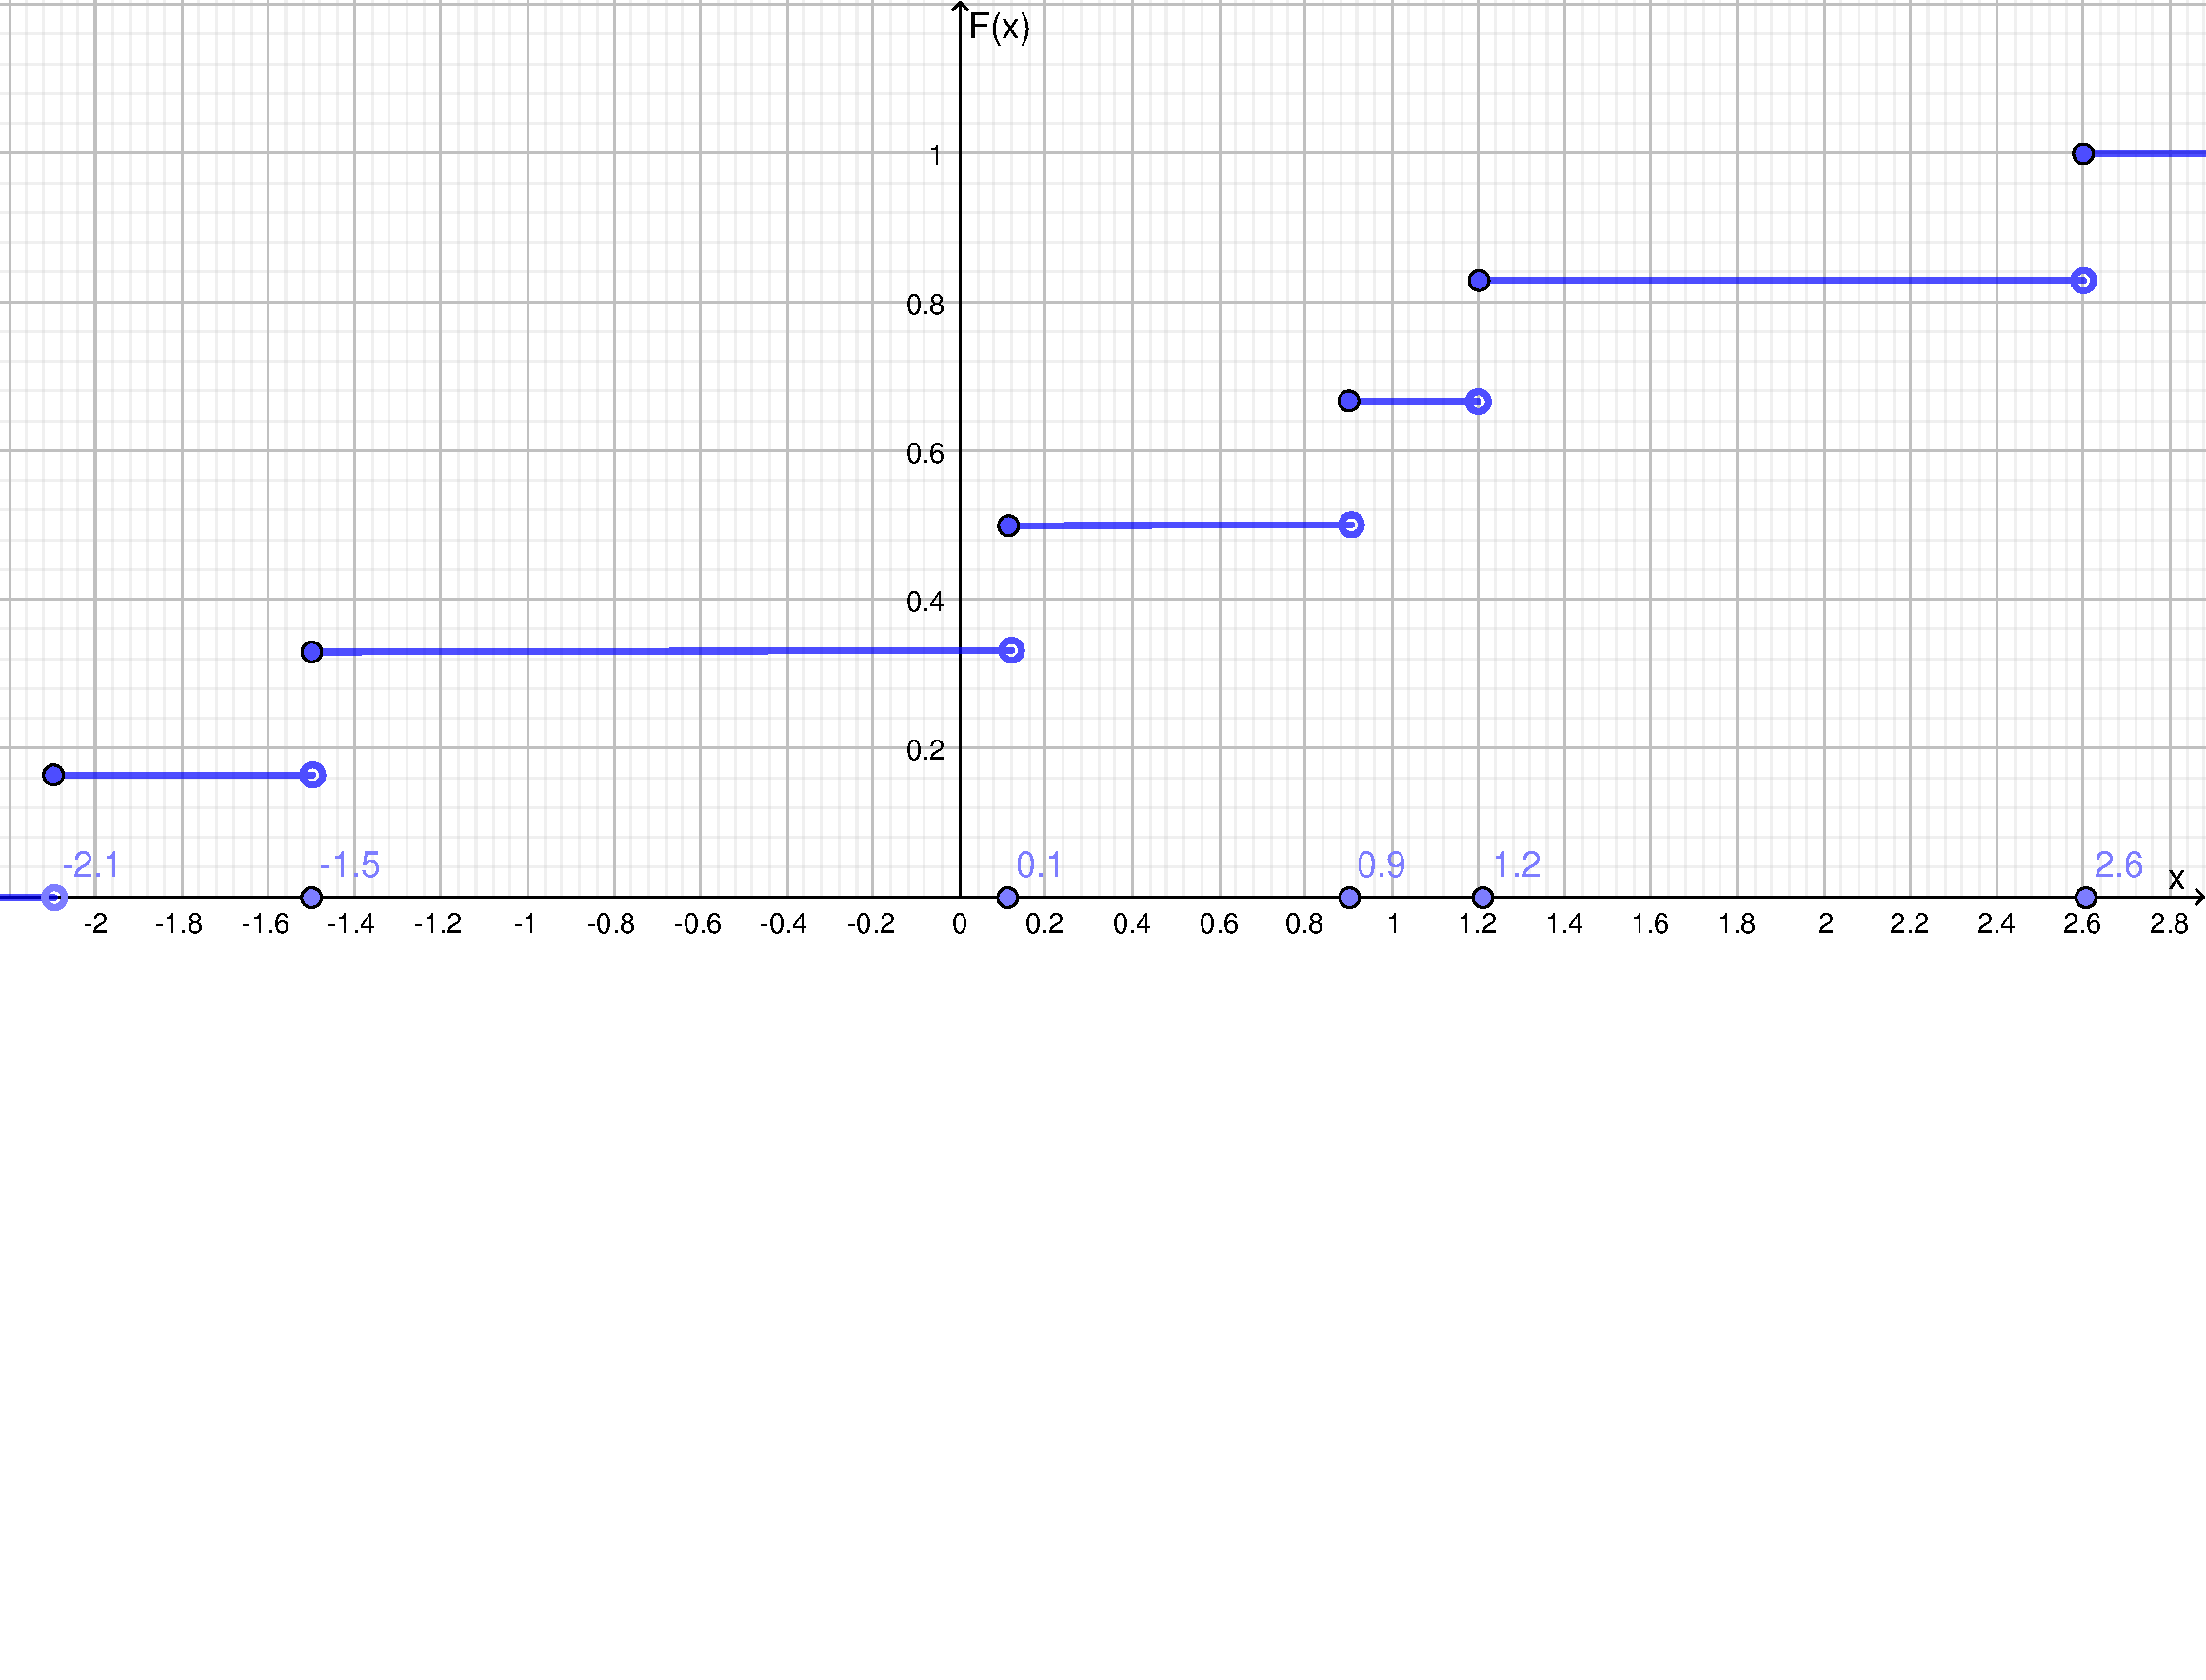
\includegraphics[scale=0.3]{func.pdf}
\end{enumerate}

\item \label{Кр4 2009-2010 №4} Кр4 2009-2010 №4. Известно, что для двух случайных величин $X$ и $Y$: $\E(X)=1$, $\E(Y)=2$, $\E(X^2)=2$, $\E(Y^2)=8$, $\E(XY)=1$.
\begin{enumerate}
\item Найдите ковариацию и коэффициент корреляции величин $X$ и $Y$.
\item Определите, зависимы ли величины $X$ и $Y$.
\item Вычислите дисперсию их суммы.
\end{enumerate}

Решение:
\begin{enumerate}
\item
\begin{align*}
\Cov (X, Y) &= \E(X \cdot Y) - \E(X) \cdot \E(Y) \\
\Cov (X, Y) &= 1-1 \cdot 2 = -1 \\
\Corr(X, Y) &= \frac{\cov(X,Y)}{\sqrt{\Var(X) \cdot \Var(Y)}} \\
\Var(X) &= \E(X^2) - (\E(X))^2  = 2 - 1^2 = 1\\
\Var(Y) &= \E(Y^2) - (\E(Y))^2  = 8 - 2^2 = 4\\
\Corr (X,Y) &= \frac{-1}{\sqrt{1 \cdot 4}} = - \frac{1}{2}
\end{align*}

\item $\cov(X,Y) \neq 0 \text{ , следовательно, } X$ и $Y$ зависимы

\begin{align*}
\Var(X + Y) &= \Var(X) + \Var(Y) + 2 \cov(X,Y) \\ 
\Var(X + Y) &= 1 + 4 + 2 \cdot (-1) = 3
\end{align*}
\end{enumerate}

\item \label{Кр4 2009-2010 №5} Кр4 2009-2010 №5. Предположим, что время «жизни» $X$ энергосберегающей лампы распределено по нормальному закону. По 10 наблюдениям среднее время «жизни» составило 1200 часов, а выборочное стандартное отклонение 120 часов.
\begin{enumerate}
\item Постройте двусторонний доверительный интервал для математического ожидания величины $X$ с уровнем доверия 0.90.
\item Постройте двусторонний доверительный интервал для стандартного отклонения величины $X$ с уровнем доверия 0.80.
\item Какова вероятность, что несмещенная оценка для дисперсии, рассчитанная по 20 наблюдениям, отклонится от истинной дисперсии меньше, чем на 40\%?
\end{enumerate}

Решение:
\begin{enumerate}

\item
$X_i \sim \cN(\mu, \sigma^2), n = 10, \bar X = 1200, \hat{\sigma} = 120$

\[
\frac{\bar X - \mu}{\hat{\sigma} / \sqrt{n}} \stackrel{}{\sim} t_{n-1}
\]
Доверительный интервал:
\[
\bar X - t_{n-1; \alpha/2} \cdot \frac{\hat{\sigma}}{\sqrt{n}} < \mu < \bar X + t_{n-1; 1 - \alpha/2} \cdot \frac{\hat{\sigma}}{\sqrt{n}}
\]
Реализация доверительного интервала:
\[
1200 - 1.83 \cdot \frac{120}{\sqrt{10}} < \mu < 1200 + 1.83 \cdot \frac{120}{\sqrt{10}}
\]
\[
1130.44 < \mu < 1269.57
\]

\item

\begin{align*}
\frac{{\hat \sigma^2}}{\sigma^2} (n-1) \stackrel{}{\sim} \chi_{n-1}^2 \\
\end{align*}

\item
\end{enumerate}

\item Кр4 2009-2010 №6. Учебная часть утверждает, что все три факультатива «Вязание крючком для экономистов», «Экономика вышивания крестиком» и «Статистические методы в макраме» одинаково популярны. В этом году на эти факультативы соответственно записалось 35, 31 и 40 человек. Правдоподобно ли заявление учебной части?\label{Кр4 2009-2010 №6}

Решение:

\begin{align*}
	H_0: p_1 &= \frac{1}{3}, p_2 = \frac{1}{3},  p_3 = \frac{1}{3} \\
	H_a: p_1 &\neq \frac{1}{3}, p_2 \neq \frac{1}{3}, p_3 \neq \frac{1}{3}
\end{align*}

\[	
W_n = \sum_{i=1}^r\frac{(\nu_i - n \cdot p_i)^2}{n \cdot p_i}\sim \chi_2^2
\]

\[
W_{obs} = \frac{(35 - 106 \cdot \frac{1}{3})^2}{106 \cdot \frac{1}{3}} + \frac{(31 - 106 \cdot \frac{1}{3})^2}{106 \cdot \frac{1}{3}} + \frac{(40 - 106 \cdot \frac{1}{3})^2}{106 \cdot \frac{1}{3}} \approx 1.15
\]
Возьмём $\alpha = 0.05$.

$W_{crit}$ находим по табличке, $W_{crit} \approx 5.99$.

Заметим, что $W_{obs} < W_{crit}$, поэтому гипотеза $H_0$ не отвергается.

\item \label{Кр4 2009-2010 №7} Кр4 2009-2010 №7. Имеются две конкурирующие гипотезы:
\begin{enumerate}
\item[$H_0$:] Случайная величина X распределена равномерно на (0,100);
\item[$H_a$:] Случайная величина X распределена равномерно на (50,150).
\end{enumerate}
Исследователь выбрал следующий критерий: если $X<c$, принимать гипотезу $H_0$, иначе  $H_a$.
\begin{align*}
	H_0&: X_i \sim \cU(0,100) \\
	H_a&: X_i \sim \cU(50,150) 
\end{align*}
\begin{enumerate}
\item Определения

\item
\begin{align*}
\P(\text{ошибка первого рода}) &= \P(X_i > c | X_i \sim \cU(0,100)) \\
\alpha =  \P(\text{ошибка первого рода}) &= \frac{100 - c}{100} = 1 - \frac{c}{100}
\end{align*}

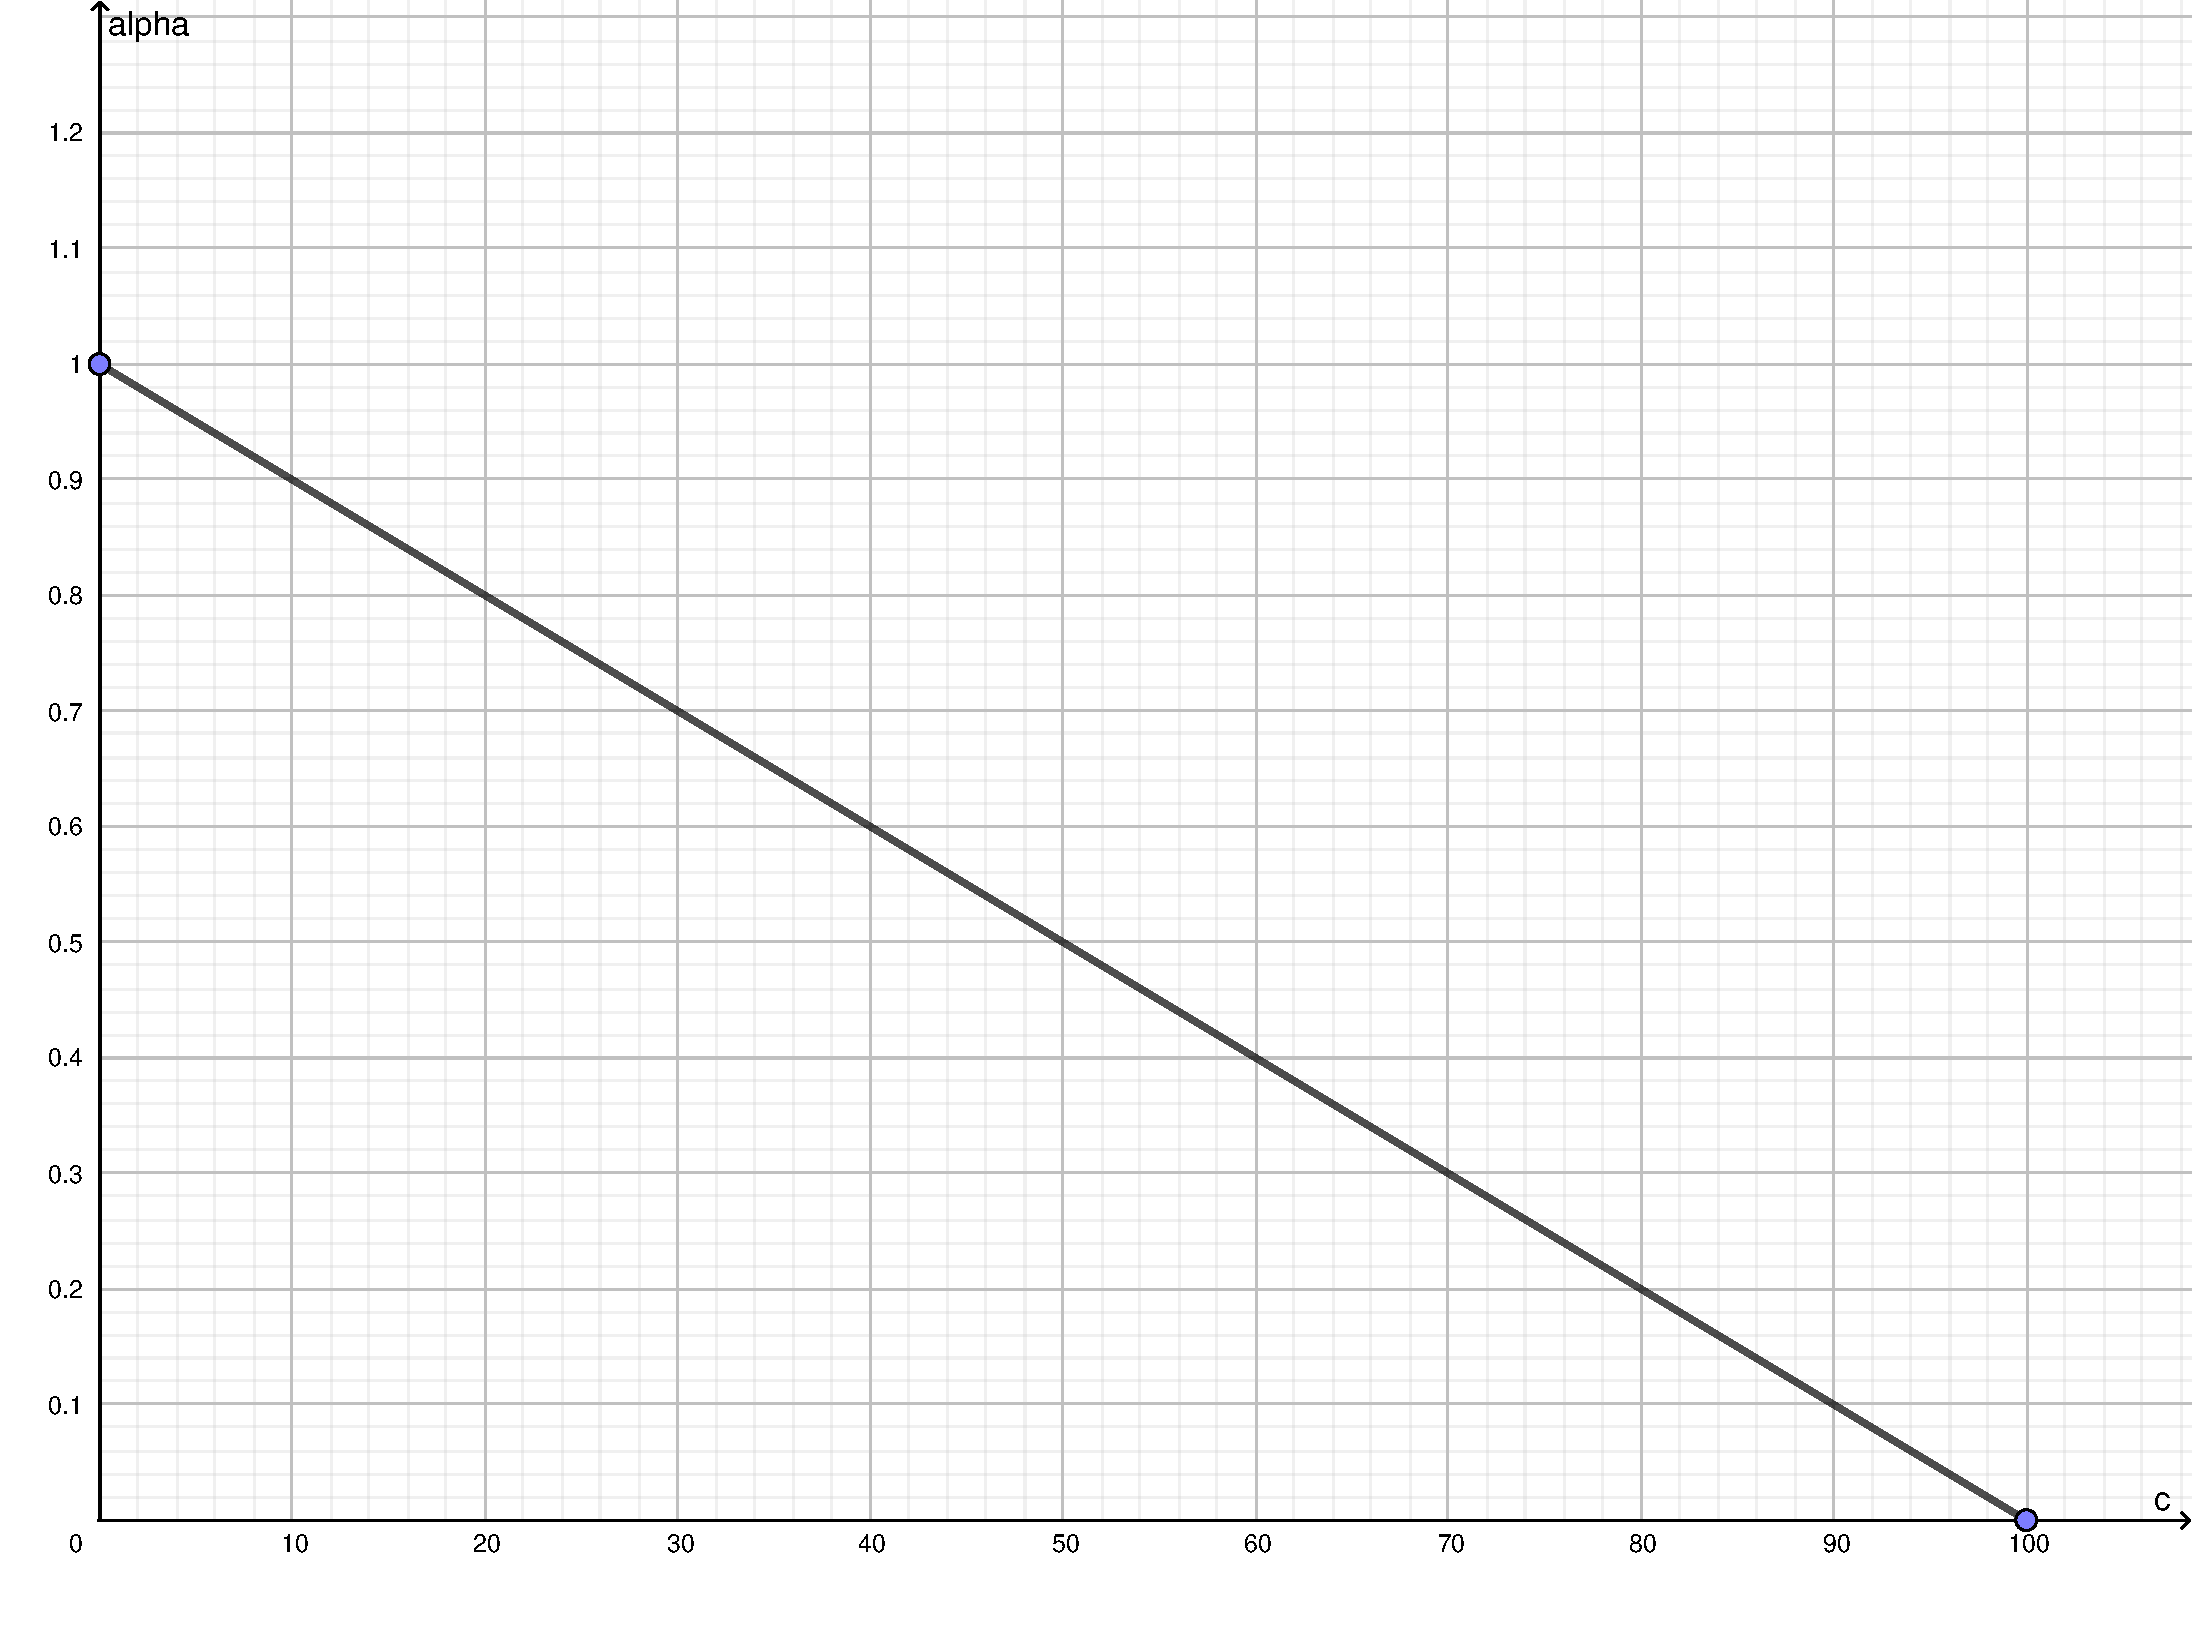
\includegraphics[scale=0.3]{1.pdf}

Видно, что график зависимости ошибки первого рода от с является прямой с отрицательным наклоном, при этом с может принимать значения от 0 до 100, поскольку вероятность принимает значения от 0 до 1.

\begin{align*}
\P(\text{ошибка второго рода}) &= \P(X_i < c | X_i \sim \cU(50,150)) \\
\beta =  \P(\text{ошибка второго рода}) &= \frac{c-50}{100} = \frac{c}{100} - \frac{1}{2}
\end{align*}

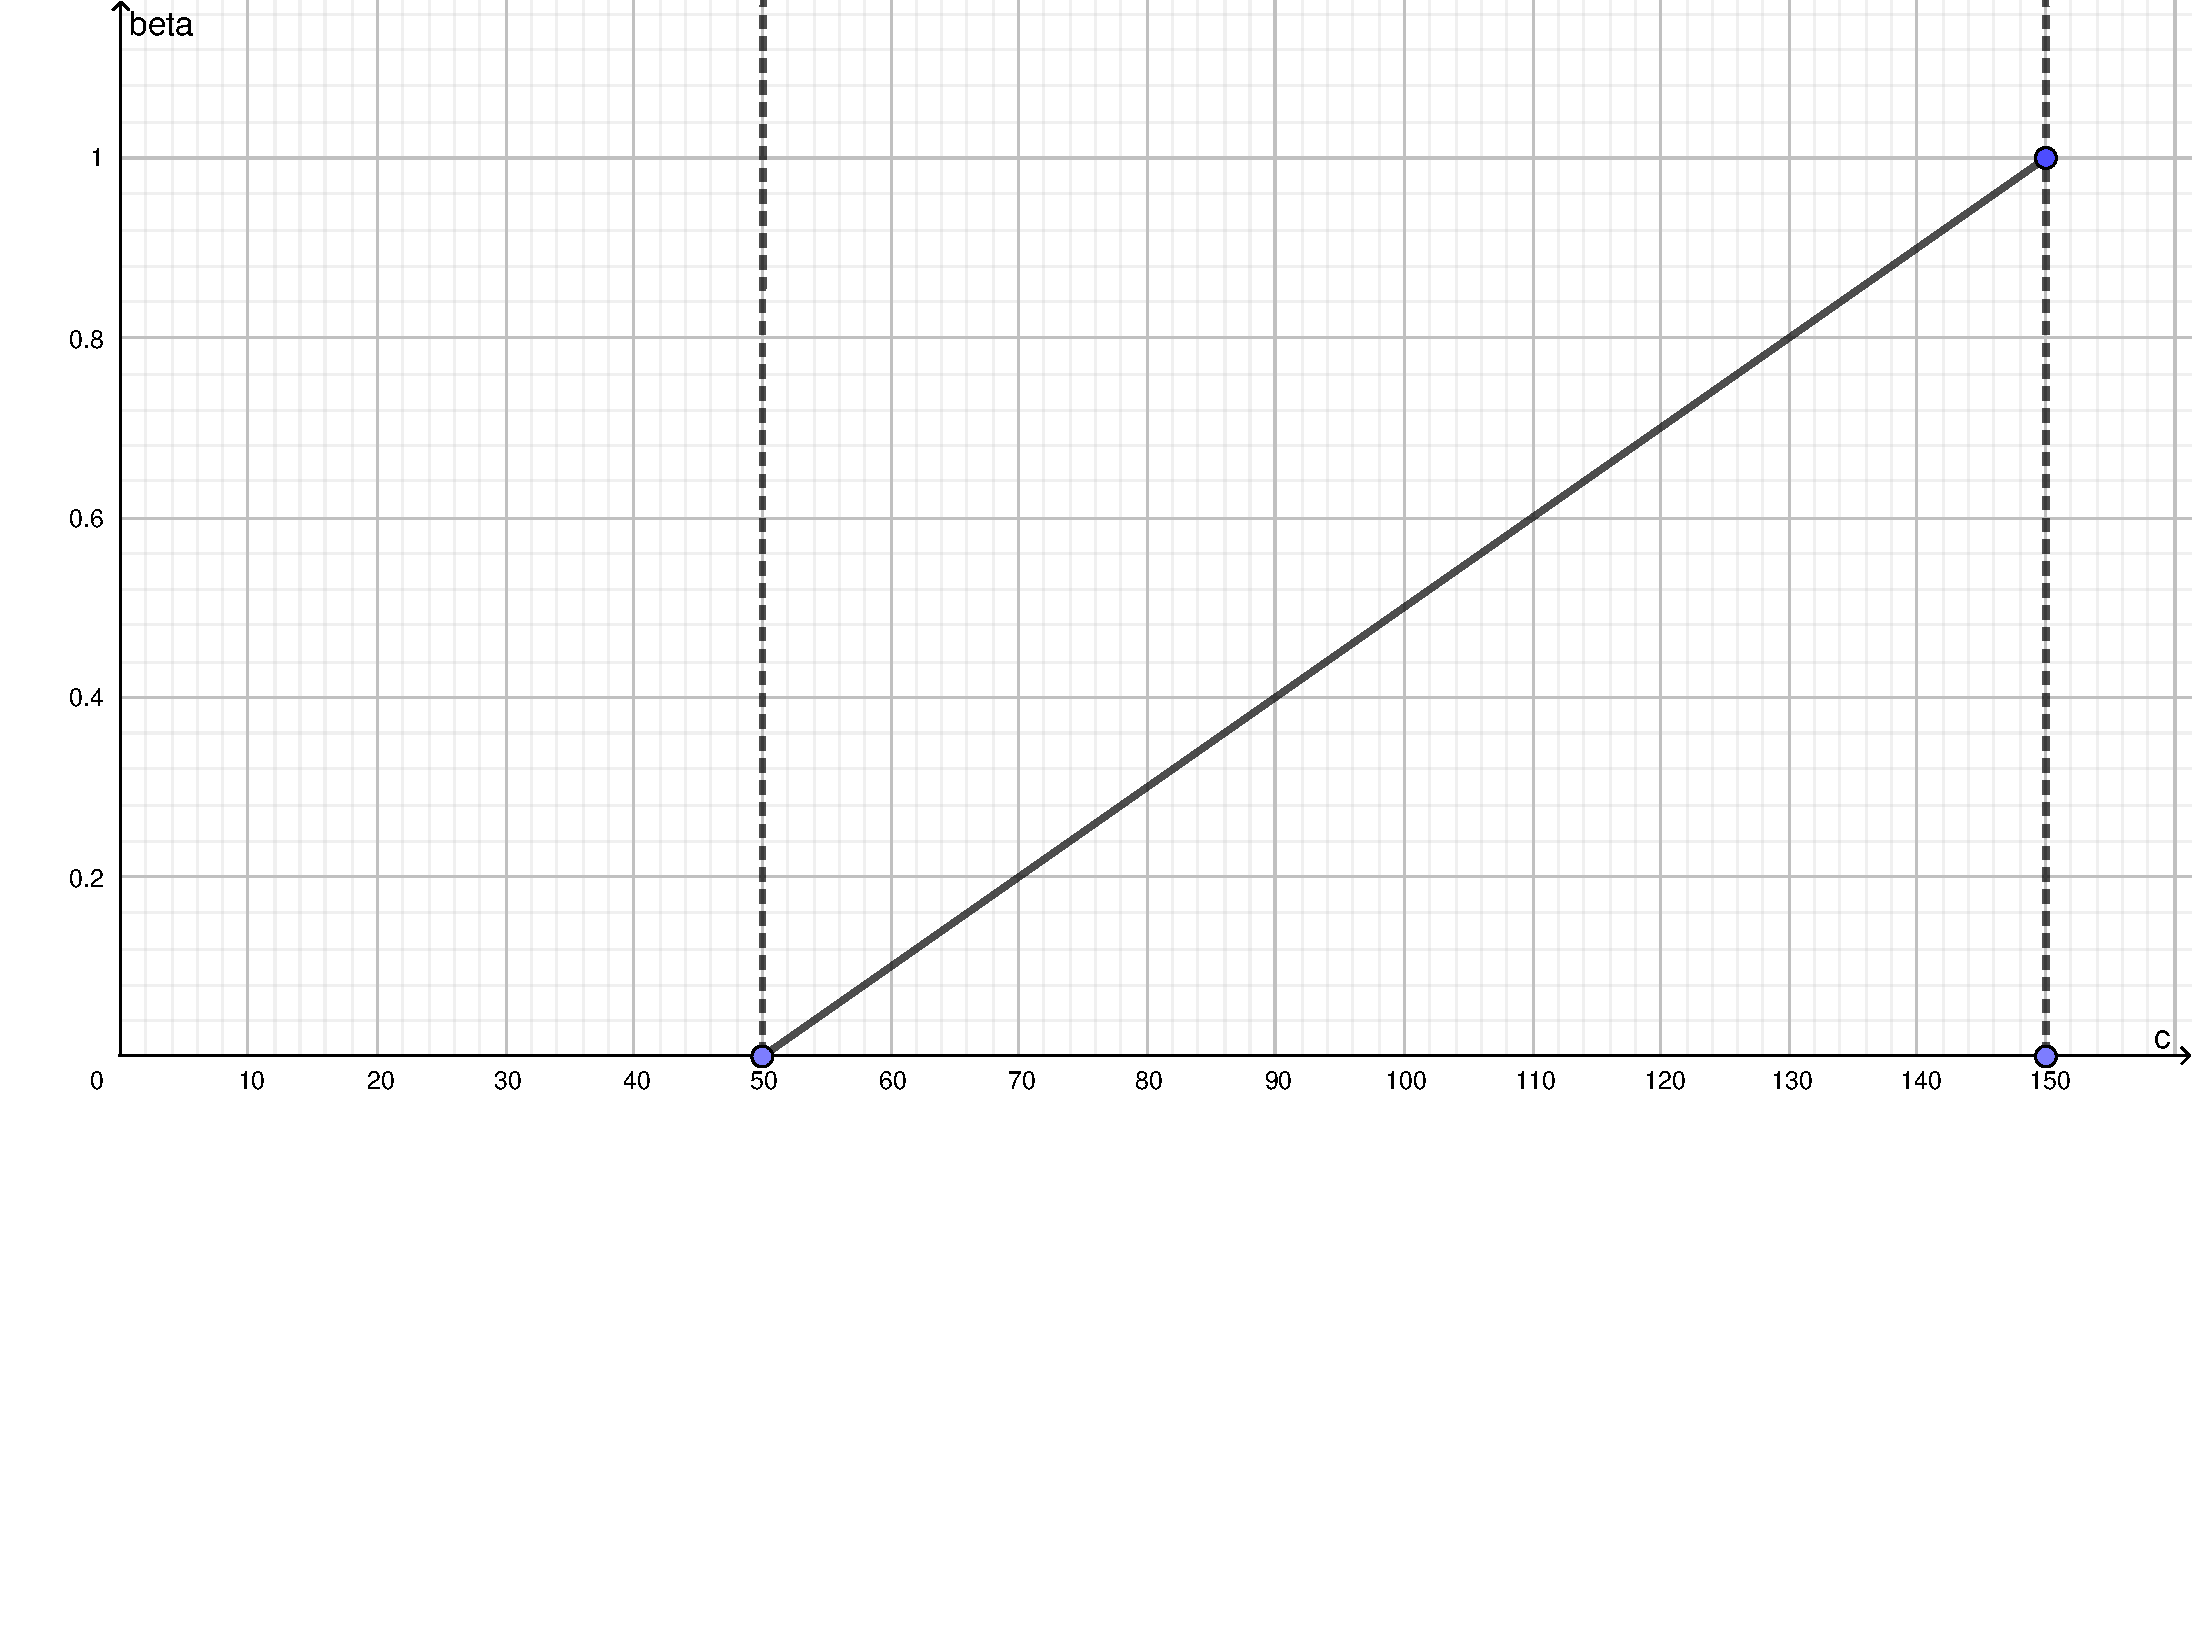
\includegraphics[scale=0.3]{2.pdf}

График зависимости ошибки второго рода от с является прямой с положительным наклоном, при этом с может принимать значения от 50 до 150, так как вероятность принимает значения от 0 до 1.

$\alpha = 0.05$
\item
\[
1 - \frac{c}{100} = 0.05 \text{ , следовательно, } \frac{c}{100} = 0.95 \text{ , следовательно, } c = 95 
\]

\[
\beta = \frac{c-50}{100} = 0.45
\]
\end{enumerate}

\item \label{Кр4 2009-2010 №9} Кр4 2009-2010 №9. Случайная величина $X$, характеризующая срок службы элементов электронной аппаратуры, имеет распределение Релея: $F(x)=1-e^{-x^2/\theta}$ при $x\geq 0$. 

По случайной выборке $X_1$, $X_2$, ..., $X_n$ найдите оценку максимального правдоподобия параметра $\theta$.

Решение:
\begin{align*}
F(x) &= 1 - e^{-x^2/\theta} \\
f(x) = F'(x) = &-e^{-x^2/\theta} \cdot \left(- \frac{2x}{\theta}\right) = x \cdot \frac{2}{\theta} \cdot e^{-x^2/\theta} 
\end{align*}

Функция правдоподобия:

\begin{align*}
L &= \prod_{i=1}^n x_i \frac{2}{\theta} e^{- \frac{x_i^2}{\theta}}  = \prod_{i=1}^n x_i \cdot \frac{2^n}{\theta^n} \cdot e^{-\frac{1}{\theta} \cdot \sum_{i=1}^n x_i^2 } \cdot   \\
\ell &= \ln L = \sum_{i=1}^n \ln x_i + n \ln 2 - n \ln\theta - \frac{1}{\theta} \cdot \sum_{i=1}^n x_i^2 \\
\end{align*}
\begin{align*}
\frac{\partial \ell}{\partial \theta} = \left. \frac{-n}{\theta} + \frac{\sum_{i=1}^n x_i^2} {\theta^2} \right|_{\theta = \hat \theta_{ML}} = 0 \\
-n \hat {\theta} + \sum_{i=1}^n x_i^2 = 0 \text{ , следовательно, } \hat \theta_{ml} = \frac{\sum_{i=1}^n X_i^2}{n} \\
\end{align*}
\[
\frac{\partial^2 \ell}{\partial \theta \partial \theta} = \frac{n}{\theta^2} - 2 \cdot \frac{\sum_{i=1} x_i^2}{\theta^3} = \frac{n\theta - 2\sum_{i=1}^n x_i^2}{\theta^3}
\]
Знаменатель $>0$. Определим знак числителя в точке $\theta = \hat{\theta_{ml}}$:
\[
n \cdot \frac{\sum_{i=1}^n x_i^2}{n} - 2 \cdot \sum_{i=1}^n x_i^2  = - \sum_{i=1}^n x_i^2 < 0 \text{ , следовательно, } максимум
\]

\item \label{Кр4 2009-2010 №10} Кр4 2009-2010 №10. По случайной выборке $X_1$, $X_2$, \ldots, $X_n$ из равномерного на интервале $[\theta;\theta+10]$ распределения методом моментов найдите оценку параметра $\theta$. Дайте определение несмещенности и состоятельности оценки и определите, будет ли обладать этими свойствами найденная оценка.

Решение:

$X_i \sim \cN(\theta; \theta + 10$

\[
\E (X_i) = \frac{\theta + (\theta + 10 )}{2} = \theta + 5
\]

\[
\hat \alpha = \frac{1}{n} \sum_{i=1}^n X_i \text{ - выборочный первый начальный момент}
\]

Найдем оценку, приравняв математическое ожидание и выборочный первый начальный момент.

\[
\hat \theta_{MM} + 5 = \frac{1}{n} \sum_{i=1}^n X_i
\]

Таким образом, получаем:
\[
\hat \theta_{MM} = \bar X - 5
\]

Оценка является несмещённой, если $\E (\hat \theta) = \theta$

\[
\E(\hat \theta) = \E(\bar X - 5) = \E(X_i) - 5 = \theta \text{ ,следовательно, не смещена}
\]
Оценка является состоятельной, если $\P(|\hat \theta - \theta| > \varepsilon) \stackrel{\P}{\rightarrow} 0$ при $n \rightarrow \infty$

Так как наша оценка не смещена, то можем использовать предел дисперсии оценки для определения состоятельности.

\[
\lim_{n\to\infty} \Var(\hat \theta) = \lim_{n\to\infty} \Var(\bar X - 5) = \lim_{n\to\infty} \frac{1}{n} \Var(X_i)
\]
\[
\Var(X_i) = \frac{((\theta + 10) - \theta)^2}{12} = 100 / 12 \\
\]
\[
\lim_{n\to\infty} \Var(\hat \theta) = \lim_{n\to\infty} \frac{1}{n} \cdot \frac{100}{12} = 0
\]

Следовательно, оценка является состоятельной.

\item \label{Кр4 2009-2010 №11} Кр4 2009-2010 №11. При расчете страхового тарифа страховая компания предполагает, что вероятность наступления страхового случая 0.005. По итогам прошедшего года из 10000 случайно выбранных договоров страховых случаев наблюдалось 67.
\begin{enumerate}
\item Согласуются ли полученные данные с предположением страховой компании? Альтернативная гипотеза: вероятность страхового случая больше.
\item Определить минимальный уровень значимости, при котором основная гипотеза отвергается.
\end{enumerate}

Решение:

\begin{enumerate}
\item
$\hat p = \frac{67}{10000} = 0.0067$

\[
X_i = \begin{cases}
	1, p \\
	0, 1-p
\end{cases}
\]

\[
\begin{cases}
	H_0 : p = 0.005 \\
	H_a : p > 0.005
\end{cases}
\]

Известно, что:
\[
\frac{\hat p - p }{\sqrt{\frac{\hat p (1- \hat p)}{n}}} \stackrel{as}{\sim} \cN(0,1)
\]

\[
Z_{obs} = \frac{0.0067 - 0.005}{\sqrt{\frac{0.0067 \cdot 0.9933}{10000}}} \approx 2.08
\]

Возьмём уровень доверия $\alpha = 0.05$
 
Гипотеза односторонняя, отсекаем только хвост справа
 
\[
Z_{crit} = Z_{1-\alpha} \approx 1.65
\]
Область, в которой $H_0$ не отвергается: $[-\infty ;1.65]$.
 
Т.к. $Z_{obs} = 2.08 > 1.65$ гипотеза $H_0$ отвергается.
 
\item
 
$p-value$ - минимальный уровень значимости, при котором гипотеза $H_0$ не отвергается. 
 
\[
p-value = \P(Z > 2.08) = 1 - \P(Z < 2.08) = 0.018
\]
\end{enumerate}



\end{enumerate}
\end{document}